\documentclass{article}
\usepackage{amsthm, amsmath, graphicx, enumitem, tikz-qtree}
\usepackage[margin=0.5in]{geometry}
\graphicspath{ {7_img/} }
\begin{document}
    \noindent\textbf{CS 373 Homework 7}\hfill Anchu A. Lee\\
    \noindent\today\\
    \begin{enumerate}
        \item Construct a pushdown automata that recognizes $\{w \mid w $ is an element of $ \{0,1\}^* $ and $w$ has more 0's than 1's $ \}$.\\
        \begin{center}
            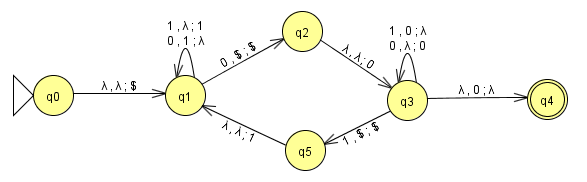
\includegraphics[scale=0.6]{machine1}
        \end{center}

        \item Convert the following CFG into an equivalent CFG in Chomsky normal form, using the procedure given in Theorem 2.9.
            \begin{align*}
                A&\rightarrow BAB\mid B\mid \epsilon\\
                B&\rightarrow 00 \mid \epsilon
            \end{align*}
            $S\rightarrow BC \mid AB \mid BA \mid BB \mid DD \mid \epsilon$\\
            $A\rightarrow BC\mid AB \mid BA \mid BB \mid DD$\\
            $B\rightarrow DD$\\
            $C\rightarrow AB$\\
            $D\rightarrow 0$
        \item Show that the class of context-free languages is closed under the union operation (construction and proof). The construction should be quite simple.
            \begin{proof}
                Define two context-free languages: $G_1=(V_1, \Sigma, R_1, S_1)$ and $G_2=(V_2, \Sigma, R_2, S_2)$ and also the language $G_U = (V_1\cup V_2\cup \{S\},\Sigma, R_1\cup R_2\cup \{S\rightarrow S_1 \mid S_2\}, S )$ which is the union of $G_1$ and $G_2$ as the start variable of $G_U$ points to both start variables of $G_1$ and $G_2$. Additionally the rules and variables are shared (assuming the rules and variables are disjoint). After the start variable of $G_U$, subsequent steps use rules exclusively from $G_1$ or $G_2$, not both. therefore all productions of $G_U$ must be in the languages $G_1$ or $G_2$.
            \end{proof}
        \item Show that the class of context-free languages is closed under the concatenation operation (construction and proof). The construction should be quite simple.
            \begin{proof}
                Define two context-free languages: $G_1=(V_1, \Sigma, R_1, S_1)$ and $G_2=(V_2, \Sigma, R_2, S_2)$ and also the language $G_C=(V_1\cup V_2\cup \{S\}, \Sigma, R_1\cup R_2\cup \{S\rightarrow S_1S_2\}, S)$ which is the concatenation of $G_1$ and $G_2$ ad the start variable of $G_C$ concatenates both the start variables of $G_1$ and $G_2$. So $G_C$ produces words that start with $G_1$ and end with $G_2$, thus all productions of $G_C$ must be concatenations of $G_1$ and $G_2$.
            \end{proof}
        \item Show that the class of context-free languages is closed under the star operation (construction and proof). The construction should be quite simple.
            \begin{proof}
                Define the context-free language $G_1=(V, \Sigma, R, S)$. The star of this language would have to be able to generate $\Sigma$ or a countably infinite amount of copies. So the start state would have to $S_0\rightarrow \epsilon \mid S_0S$. Therefore the language $G_S=(V, \Sigma, R \cup \{S_0\rightarrow\epsilon\mid S_0S\}, S_0)$ generates either $\epsilon$ or a sequence of many words in $G_1$.
            \end{proof}
        \item Let $M=(Q,\Sigma, \delta, q_0, F)$ be a DFA and define CFG $G=(V,\Sigma,R,S)$ as follows:
            \begin{itemize}
                \item $V = Q$;
                \item For each $q\in Q$ and $ a\in \Sigma $, define rule $q\rightarrow aq'$ where $q'=\delta(q,a)$;
                \item For $q\in F$ define rule $q\rightarrow\epsilon$;
                \item $S=q_0$.
            \end{itemize}
            Prove $L(M) = L(G)$.
            \begin{proof}
                A language is regular if a DFA accepts it, so $L(M)$ is a regular language. By Corollary 2.32, the language must also be context-free. In order for $L(M) = L(G)$, the construction of $G$ must be a direct translation of a DFA to GFA. $G$ converts the states of a DFA to variables, defines rules that function similarly to the transition functions and uses a rule that moves to $\epsilon$ instead of using accept states. This construction successfully translates a DFA into a CFG.
            \end{proof}
        \item Let $L=\{0^n1^m0^n1^m \mid n,m \geq 0\}$. Show $L$ is not context-free.
            \begin{proof}
                Assume $L$ is context-free. Let $p$ be the pumping length. Let $w=0^p1^p0^p1^p$, which means the options for $vxy$ are $0^p$, $0^p1^p$, $1^p$, $1^p0^p$. Each option is really two options as the string is $0^p1^p$ twice. If $0^p$ is pumped up, then there will be too many characters in one of the zero's. If $0^p1^p$ is pumped up, then the left side of the word will be longer than the right side. If $1^p$ is pumped up then one of 1's will have too many characters than the other 1's. If $1^p0^p$ is pumped up then the middle two 1's and 0's will be larger than the outer 1's and 0's when they need to be equal. Since every case of $uvxyz0$ is not in $L$, the language cannot be context-free. 
            \end{proof}
        \item Let $L=\{w\mid w $ is in $\{a,b,c,d\}^*$, with the number of a's = number of b's and the number of c's = the number of d's $\}$. Show $L$ is not context-free.

        \item Let $A$ and $B$ be languages. We define $A\approx B = \{ab \mid a $ is an element of $A$ and $b$ is an element of $B$ and $|a| > |b|$ $\}$. Show that if $A$ and $B$ are regular languages, then $A\approx B$ is a context free language.

        \item Show $L = \{w\mid w $is an element of $\{a,b,c,d,e,f\}^*$ such that the number of a's + number of b's = number of c's + number of d's = number of e's + number of f's$ \}$ is not context-free.
    \end{enumerate}
\end{document}